% Options for packages loaded elsewhere
\PassOptionsToPackage{unicode}{hyperref}
\PassOptionsToPackage{hyphens}{url}
%
\documentclass[
]{article}
\usepackage{lmodern}
\usepackage{amssymb,amsmath}
\usepackage{ifxetex,ifluatex}
\ifnum 0\ifxetex 1\fi\ifluatex 1\fi=0 % if pdftex
  \usepackage[T1]{fontenc}
  \usepackage[utf8]{inputenc}
  \usepackage{textcomp} % provide euro and other symbols
\else % if luatex or xetex
  \usepackage{unicode-math}
  \defaultfontfeatures{Scale=MatchLowercase}
  \defaultfontfeatures[\rmfamily]{Ligatures=TeX,Scale=1}
\fi
% Use upquote if available, for straight quotes in verbatim environments
\IfFileExists{upquote.sty}{\usepackage{upquote}}{}
\IfFileExists{microtype.sty}{% use microtype if available
  \usepackage[]{microtype}
  \UseMicrotypeSet[protrusion]{basicmath} % disable protrusion for tt fonts
}{}
\makeatletter
\@ifundefined{KOMAClassName}{% if non-KOMA class
  \IfFileExists{parskip.sty}{%
    \usepackage{parskip}
  }{% else
    \setlength{\parindent}{0pt}
    \setlength{\parskip}{6pt plus 2pt minus 1pt}}
}{% if KOMA class
  \KOMAoptions{parskip=half}}
\makeatother
\usepackage{xcolor}
\IfFileExists{xurl.sty}{\usepackage{xurl}}{} % add URL line breaks if available
\IfFileExists{bookmark.sty}{\usepackage{bookmark}}{\usepackage{hyperref}}
\hypersetup{
  pdftitle={Comparative effectiveness studies data model},
  pdfauthor={Martijn J. Schuemie},
  hidelinks,
  pdfcreator={LaTeX via pandoc}}
\urlstyle{same} % disable monospaced font for URLs
\usepackage[margin=1in]{geometry}
\usepackage{longtable,booktabs}
% Correct order of tables after \paragraph or \subparagraph
\usepackage{etoolbox}
\makeatletter
\patchcmd\longtable{\par}{\if@noskipsec\mbox{}\fi\par}{}{}
\makeatother
% Allow footnotes in longtable head/foot
\IfFileExists{footnotehyper.sty}{\usepackage{footnotehyper}}{\usepackage{footnote}}
\makesavenoteenv{longtable}
\usepackage{graphicx,grffile}
\makeatletter
\def\maxwidth{\ifdim\Gin@nat@width>\linewidth\linewidth\else\Gin@nat@width\fi}
\def\maxheight{\ifdim\Gin@nat@height>\textheight\textheight\else\Gin@nat@height\fi}
\makeatother
% Scale images if necessary, so that they will not overflow the page
% margins by default, and it is still possible to overwrite the defaults
% using explicit options in \includegraphics[width, height, ...]{}
\setkeys{Gin}{width=\maxwidth,height=\maxheight,keepaspectratio}
% Set default figure placement to htbp
\makeatletter
\def\fps@figure{htbp}
\makeatother
\setlength{\emergencystretch}{3em} % prevent overfull lines
\providecommand{\tightlist}{%
  \setlength{\itemsep}{0pt}\setlength{\parskip}{0pt}}
\setcounter{secnumdepth}{5}

\title{Comparative effectiveness studies data model}
\author{Martijn J. Schuemie}
\date{2020-02-19}

\begin{document}
\maketitle

{
\setcounter{tocdepth}{2}
\tableofcontents
}
This document describes the data model for storing the output of the
comparative effectiveness analyses.

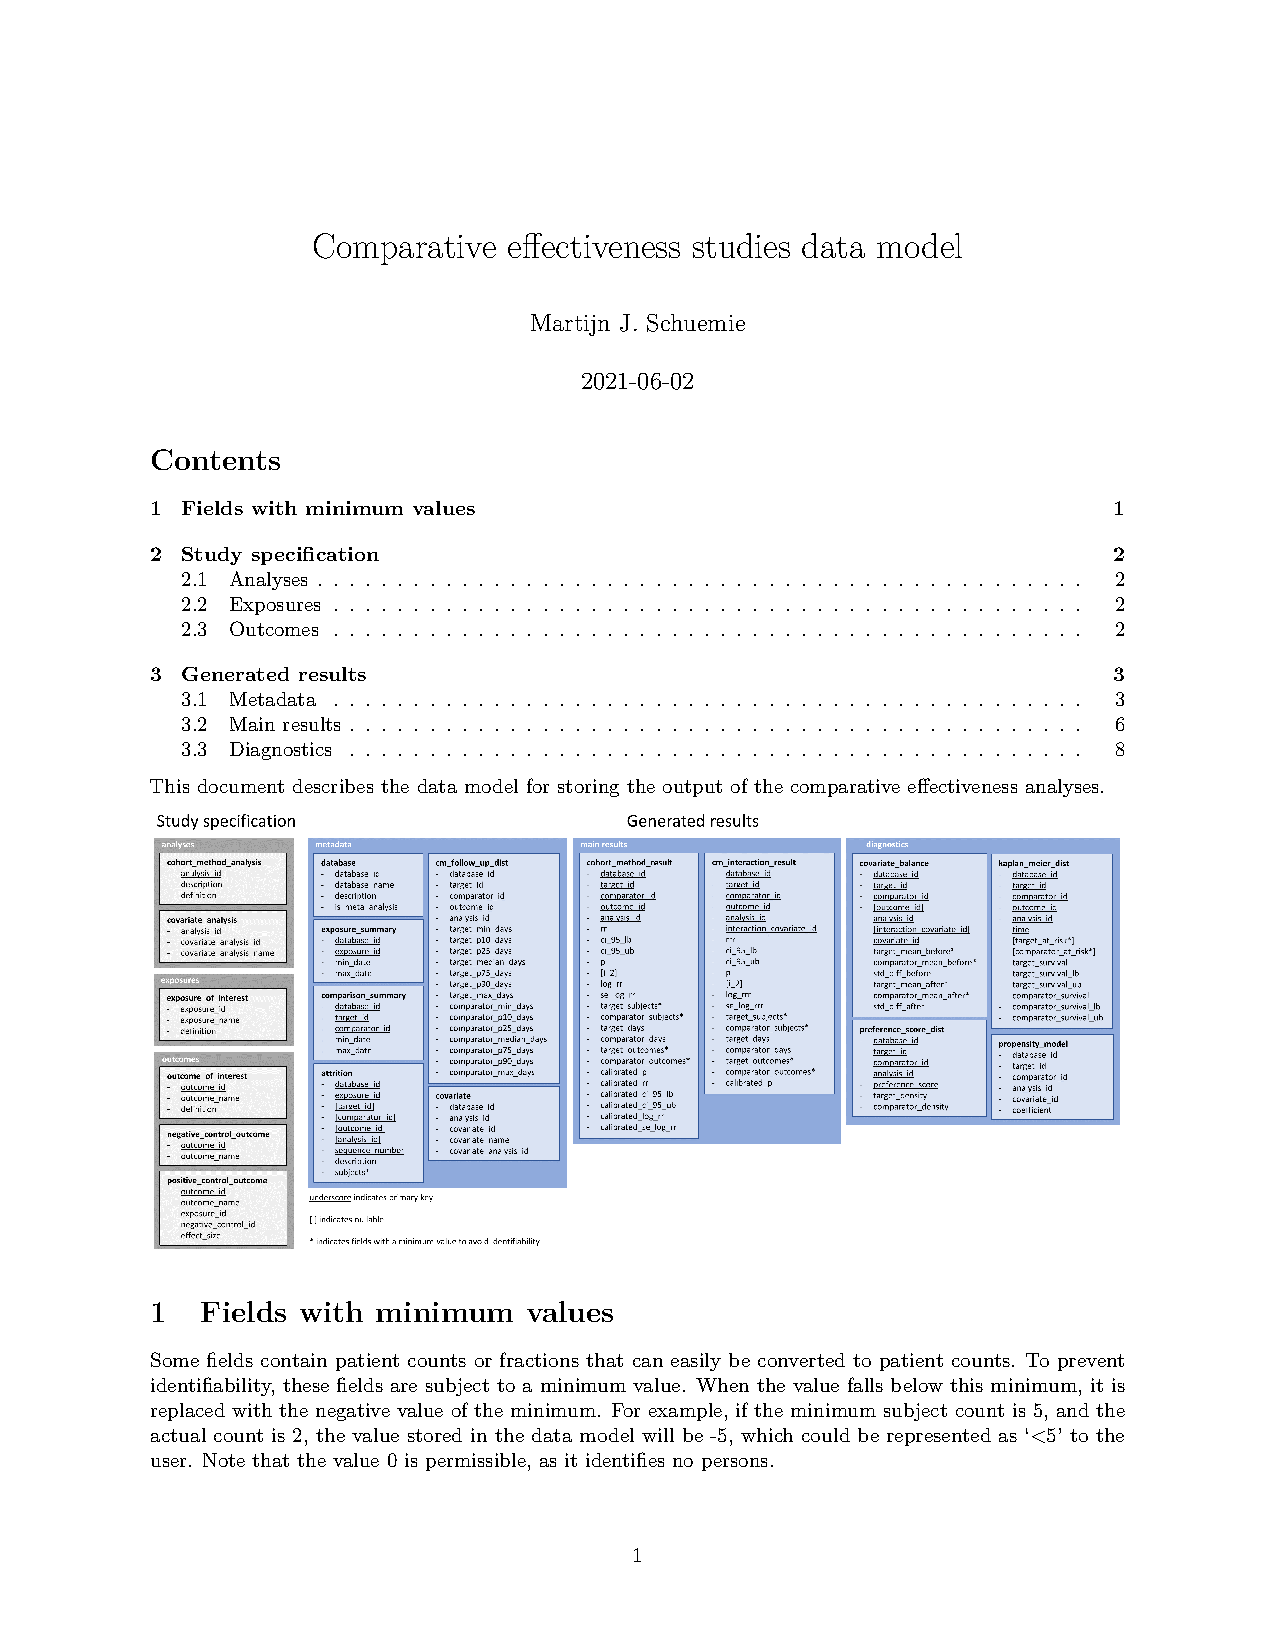
\includegraphics{DataModel.png}

\hypertarget{fields-with-minimum-values}{%
\section{Fields with minimum values}\label{fields-with-minimum-values}}

Some fields contain patient counts or fractions that can easily be
converted to patient counts. To prevent identifiability, these fields
are subject to a minimum value. When the value falls below this minimum,
it is replaced with the negative value of the minimum. For example, if
the minimum subject count is 5, and the actual count is 2, the value
stored in the data model will be -5, which could be represented as
`\textless5' to the user. Note that the value 0 is permissible, as it
identifies no persons.

These fields have been marked with * in the preceding diagram, and are
noted `with min value' in the Type column in the table definitions
below.

\hypertarget{study-specification}{%
\section{Study specification}\label{study-specification}}

The first set of tables are not specific to a database, but rather
provide a reference for linking results generated in databases. These
can be thought of as the study specifications.

\hypertarget{analyses}{%
\subsection{Analyses}\label{analyses}}

\hypertarget{table-cohort_method_analysis}{%
\subsubsection{Table:
cohort\_method\_analysis}\label{table-cohort_method_analysis}}

Lists the analyses that will be executed by the CohortMethod package.

\begin{longtable}[]{@{}lll@{}}
\toprule
Field & Type & Description\tabularnewline
\midrule
\endhead
analysis\_id & integer & A unique identifier for an
analysis.\tabularnewline
description & varchar & A description for an analysis,
e.g.~`On-treatment'.\tabularnewline
definition & varchar & A CohortMethod JSON object specifying the
analysis.\tabularnewline
\bottomrule
\end{longtable}

\hypertarget{table-covariate_analysis}{%
\subsubsection{Table:
covariate\_analysis}\label{table-covariate_analysis}}

Lists the covariate analyses that will be executed by the
FeatureExtraction package. Each analysis can generate one or more
covariates. For example, the age group analysis creates binary
covariates for each 5-year age group.

\begin{longtable}[]{@{}lll@{}}
\toprule
\begin{minipage}[b]{0.23\columnwidth}\raggedright
Field\strut
\end{minipage} & \begin{minipage}[b]{0.18\columnwidth}\raggedright
Type\strut
\end{minipage} & \begin{minipage}[b]{0.50\columnwidth}\raggedright
Description\strut
\end{minipage}\tabularnewline
\midrule
\endhead
\begin{minipage}[t]{0.23\columnwidth}\raggedright
analysis\_id\strut
\end{minipage} & \begin{minipage}[t]{0.18\columnwidth}\raggedright
integer\strut
\end{minipage} & \begin{minipage}[t]{0.50\columnwidth}\raggedright
A foreign key referencing the cohort\_method\_analysis table.\strut
\end{minipage}\tabularnewline
\begin{minipage}[t]{0.23\columnwidth}\raggedright
covariate\_analysis\_id\strut
\end{minipage} & \begin{minipage}[t]{0.18\columnwidth}\raggedright
integer\strut
\end{minipage} & \begin{minipage}[t]{0.50\columnwidth}\raggedright
A unique identifier for a covariate analysis.\strut
\end{minipage}\tabularnewline
\begin{minipage}[t]{0.23\columnwidth}\raggedright
covariate\_analysis\_name\strut
\end{minipage} & \begin{minipage}[t]{0.18\columnwidth}\raggedright
varchar\strut
\end{minipage} & \begin{minipage}[t]{0.50\columnwidth}\raggedright
A name for a covariate analysis, e.g.~`Demographics: age group'.\strut
\end{minipage}\tabularnewline
\bottomrule
\end{longtable}

\hypertarget{exposures}{%
\subsection{Exposures}\label{exposures}}

Exposures can be exposures to drugs, procedures, or combinations of
these. The exposure IDs used in the two exposure-of-interest tables do
not overlap.

\hypertarget{table-exposure_of_interest}{%
\subsubsection{Table:
exposure\_of\_interest}\label{table-exposure_of_interest}}

Lists all exposure cohorts considered in the study.

\begin{longtable}[]{@{}lll@{}}
\toprule
\begin{minipage}[b]{0.23\columnwidth}\raggedright
Field\strut
\end{minipage} & \begin{minipage}[b]{0.18\columnwidth}\raggedright
Type\strut
\end{minipage} & \begin{minipage}[b]{0.50\columnwidth}\raggedright
Description\strut
\end{minipage}\tabularnewline
\midrule
\endhead
\begin{minipage}[t]{0.23\columnwidth}\raggedright
exposure\_id\strut
\end{minipage} & \begin{minipage}[t]{0.18\columnwidth}\raggedright
integer\strut
\end{minipage} & \begin{minipage}[t]{0.50\columnwidth}\raggedright
A unique identifier for an exposure.\strut
\end{minipage}\tabularnewline
\begin{minipage}[t]{0.23\columnwidth}\raggedright
exposure\_name\strut
\end{minipage} & \begin{minipage}[t]{0.18\columnwidth}\raggedright
varchar\strut
\end{minipage} & \begin{minipage}[t]{0.50\columnwidth}\raggedright
A name for the exposure, e.g.~`Sertraline'.\strut
\end{minipage}\tabularnewline
\begin{minipage}[t]{0.23\columnwidth}\raggedright
definition\strut
\end{minipage} & \begin{minipage}[t]{0.18\columnwidth}\raggedright
varchar\strut
\end{minipage} & \begin{minipage}[t]{0.50\columnwidth}\raggedright
ATLAS cohort definition JSON for constructing the exposure cohort.\strut
\end{minipage}\tabularnewline
\bottomrule
\end{longtable}

\hypertarget{outcomes}{%
\subsection{Outcomes}\label{outcomes}}

Outcomes can be distinguished into outcomes of interest, where the true
effect size is unknown and of interest, negative control outcomes where
the true effect size is known to be 1, and positive control outcomes
where the true effect size is of a known magnitude greater than 1. The
outcome IDs used in the three outcome tables do not overlap.

\hypertarget{table-outcome_of_interest}{%
\subsubsection{Table:
outcome\_of\_interest}\label{table-outcome_of_interest}}

\begin{longtable}[]{@{}lll@{}}
\toprule
Field & Type & Description\tabularnewline
\midrule
\endhead
outcome\_id & integer & A unique identifier for an
outcome.\tabularnewline
outcome\_name & varchar & A name for the outcome,
e.g.~'Stroke.\tabularnewline
definition & varchar & OHDSI SQL or JSON object defining the
outcome.\tabularnewline
\bottomrule
\end{longtable}

\hypertarget{table-negative_control_outcomes}{%
\subsubsection{Table:
negative\_control\_outcomes}\label{table-negative_control_outcomes}}

Negative control outcomes are derived from a single concept ID.

\begin{longtable}[]{@{}lll@{}}
\toprule
Field & Type & Description\tabularnewline
\midrule
\endhead
outcome\_id & integer & A unique identifier for an
outcome.\tabularnewline
outcome\_name & varchar & A name for the outcome, e.g.~`Ingrown
nail'.\tabularnewline
\bottomrule
\end{longtable}

\hypertarget{table-positive_control_outcomes}{%
\subsubsection{Table:
positive\_control\_outcomes}\label{table-positive_control_outcomes}}

Positive controls are synthesized by injecting simulated outcomes into
negative controls.

\begin{longtable}[]{@{}lll@{}}
\toprule
\begin{minipage}[b]{0.23\columnwidth}\raggedright
Field\strut
\end{minipage} & \begin{minipage}[b]{0.18\columnwidth}\raggedright
Type\strut
\end{minipage} & \begin{minipage}[b]{0.50\columnwidth}\raggedright
Description\strut
\end{minipage}\tabularnewline
\midrule
\endhead
\begin{minipage}[t]{0.23\columnwidth}\raggedright
outcome\_id\strut
\end{minipage} & \begin{minipage}[t]{0.18\columnwidth}\raggedright
integer\strut
\end{minipage} & \begin{minipage}[t]{0.50\columnwidth}\raggedright
A unique identifier for an outcome.\strut
\end{minipage}\tabularnewline
\begin{minipage}[t]{0.23\columnwidth}\raggedright
outcome\_name\strut
\end{minipage} & \begin{minipage}[t]{0.18\columnwidth}\raggedright
varchar\strut
\end{minipage} & \begin{minipage}[t]{0.50\columnwidth}\raggedright
A name for the outcome, e.g.~`Ingrown nail RR=2'.\strut
\end{minipage}\tabularnewline
\begin{minipage}[t]{0.23\columnwidth}\raggedright
exposure\_id\strut
\end{minipage} & \begin{minipage}[t]{0.18\columnwidth}\raggedright
integer\strut
\end{minipage} & \begin{minipage}[t]{0.50\columnwidth}\raggedright
The exposure for which the signal is injected. A foreign key referencing
the exposure\_of\_interest table.\strut
\end{minipage}\tabularnewline
\begin{minipage}[t]{0.23\columnwidth}\raggedright
negative\_control\_id\strut
\end{minipage} & \begin{minipage}[t]{0.18\columnwidth}\raggedright
integer\strut
\end{minipage} & \begin{minipage}[t]{0.50\columnwidth}\raggedright
The negative control used to create the positive control. A foreign key
referencing outcome\_id field in the negative\_control\_outcomes
table.\strut
\end{minipage}\tabularnewline
\begin{minipage}[t]{0.23\columnwidth}\raggedright
effect\_size\strut
\end{minipage} & \begin{minipage}[t]{0.18\columnwidth}\raggedright
float\strut
\end{minipage} & \begin{minipage}[t]{0.50\columnwidth}\raggedright
The simulated effect size for the positive control.\strut
\end{minipage}\tabularnewline
\bottomrule
\end{longtable}

\hypertarget{generated-results}{%
\section{Generated results}\label{generated-results}}

The second set of tables contain the results generated on each database.

\hypertarget{metadata}{%
\subsection{Metadata}\label{metadata}}

For each database, some meta data is captured.

\hypertarget{table-database}{%
\subsubsection{Table: database}\label{table-database}}

Lists the databases that have contributed data. To identify
meta-analyses estimates across databases, a dummy database record is
created where the is\_meta\_analysis flag is set to 1.

\begin{longtable}[]{@{}lll@{}}
\toprule
\begin{minipage}[b]{0.23\columnwidth}\raggedright
Field\strut
\end{minipage} & \begin{minipage}[b]{0.18\columnwidth}\raggedright
Type\strut
\end{minipage} & \begin{minipage}[b]{0.50\columnwidth}\raggedright
Description\strut
\end{minipage}\tabularnewline
\midrule
\endhead
\begin{minipage}[t]{0.23\columnwidth}\raggedright
database\_id\strut
\end{minipage} & \begin{minipage}[t]{0.18\columnwidth}\raggedright
varchar\strut
\end{minipage} & \begin{minipage}[t]{0.50\columnwidth}\raggedright
A unique identifier for a database, e.g.~`MDCD'.\strut
\end{minipage}\tabularnewline
\begin{minipage}[t]{0.23\columnwidth}\raggedright
database\_name\strut
\end{minipage} & \begin{minipage}[t]{0.18\columnwidth}\raggedright
varchar\strut
\end{minipage} & \begin{minipage}[t]{0.50\columnwidth}\raggedright
The full name for the database, e.g.~`Truven MarketScan Multi-state
Medicaid (MDCD)'.\strut
\end{minipage}\tabularnewline
\begin{minipage}[t]{0.23\columnwidth}\raggedright
description\strut
\end{minipage} & \begin{minipage}[t]{0.18\columnwidth}\raggedright
varchar\strut
\end{minipage} & \begin{minipage}[t]{0.50\columnwidth}\raggedright
A longer description, e.g.~`Truven Health MarketScan® Multi-State
Medicaid Database (MDCD) adjudicated US health insurance claims for
Medicaid enrollees from multiple states \ldots{}'\strut
\end{minipage}\tabularnewline
\begin{minipage}[t]{0.23\columnwidth}\raggedright
is\_meta\_analysis\strut
\end{minipage} & \begin{minipage}[t]{0.18\columnwidth}\raggedright
integer\strut
\end{minipage} & \begin{minipage}[t]{0.50\columnwidth}\raggedright
Does the record pertain a meta-analysis across databases? (0=no,
1=yes)\strut
\end{minipage}\tabularnewline
\bottomrule
\end{longtable}

\hypertarget{table-exposure_summary}{%
\subsubsection{Table: exposure\_summary}\label{table-exposure_summary}}

Provides summary statistics for the exposure cohorts, independent of
other exposure cohorts.

\begin{longtable}[]{@{}lll@{}}
\toprule
\begin{minipage}[b]{0.23\columnwidth}\raggedright
Field\strut
\end{minipage} & \begin{minipage}[b]{0.18\columnwidth}\raggedright
Type\strut
\end{minipage} & \begin{minipage}[b]{0.50\columnwidth}\raggedright
Description\strut
\end{minipage}\tabularnewline
\midrule
\endhead
\begin{minipage}[t]{0.23\columnwidth}\raggedright
database\_id\strut
\end{minipage} & \begin{minipage}[t]{0.18\columnwidth}\raggedright
varchar\strut
\end{minipage} & \begin{minipage}[t]{0.50\columnwidth}\raggedright
Foreign key referencing the database.\strut
\end{minipage}\tabularnewline
\begin{minipage}[t]{0.23\columnwidth}\raggedright
exposure\_id\strut
\end{minipage} & \begin{minipage}[t]{0.18\columnwidth}\raggedright
integer\strut
\end{minipage} & \begin{minipage}[t]{0.50\columnwidth}\raggedright
A foreign key referencing the exposure\_of\_interest table.\strut
\end{minipage}\tabularnewline
\begin{minipage}[t]{0.23\columnwidth}\raggedright
min\_date\strut
\end{minipage} & \begin{minipage}[t]{0.18\columnwidth}\raggedright
date\strut
\end{minipage} & \begin{minipage}[t]{0.50\columnwidth}\raggedright
The earliest date when the exposure was observed in the database.\strut
\end{minipage}\tabularnewline
\begin{minipage}[t]{0.23\columnwidth}\raggedright
max\_date\strut
\end{minipage} & \begin{minipage}[t]{0.18\columnwidth}\raggedright
date\strut
\end{minipage} & \begin{minipage}[t]{0.50\columnwidth}\raggedright
The latest date when the exposure was observed in the database.\strut
\end{minipage}\tabularnewline
\bottomrule
\end{longtable}

\hypertarget{table-comparison_summary}{%
\subsubsection{Table:
comparison\_summary}\label{table-comparison_summary}}

Provides summary statistics for the comparison between two exposure
cohorts.

\begin{longtable}[]{@{}lll@{}}
\toprule
\begin{minipage}[b]{0.23\columnwidth}\raggedright
Field\strut
\end{minipage} & \begin{minipage}[b]{0.18\columnwidth}\raggedright
Type\strut
\end{minipage} & \begin{minipage}[b]{0.50\columnwidth}\raggedright
Description\strut
\end{minipage}\tabularnewline
\midrule
\endhead
\begin{minipage}[t]{0.23\columnwidth}\raggedright
database\_id\strut
\end{minipage} & \begin{minipage}[t]{0.18\columnwidth}\raggedright
varchar\strut
\end{minipage} & \begin{minipage}[t]{0.50\columnwidth}\raggedright
Foreign key referencing the database.\strut
\end{minipage}\tabularnewline
\begin{minipage}[t]{0.23\columnwidth}\raggedright
target\_id\strut
\end{minipage} & \begin{minipage}[t]{0.18\columnwidth}\raggedright
integer\strut
\end{minipage} & \begin{minipage}[t]{0.50\columnwidth}\raggedright
A foreign key referencing the exposure\_of\_interest table.\strut
\end{minipage}\tabularnewline
\begin{minipage}[t]{0.23\columnwidth}\raggedright
comparator\_id\strut
\end{minipage} & \begin{minipage}[t]{0.18\columnwidth}\raggedright
integer\strut
\end{minipage} & \begin{minipage}[t]{0.50\columnwidth}\raggedright
A foreign key referencing the exposure\_of\_interest table.\strut
\end{minipage}\tabularnewline
\begin{minipage}[t]{0.23\columnwidth}\raggedright
min\_date\strut
\end{minipage} & \begin{minipage}[t]{0.18\columnwidth}\raggedright
date\strut
\end{minipage} & \begin{minipage}[t]{0.50\columnwidth}\raggedright
The earliest date when both target and comparator were observed in the
database.\strut
\end{minipage}\tabularnewline
\begin{minipage}[t]{0.23\columnwidth}\raggedright
max\_date\strut
\end{minipage} & \begin{minipage}[t]{0.18\columnwidth}\raggedright
date\strut
\end{minipage} & \begin{minipage}[t]{0.50\columnwidth}\raggedright
The latest date when both target and comparator were observed in the
database.\strut
\end{minipage}\tabularnewline
\bottomrule
\end{longtable}

\hypertarget{table-attrition}{%
\subsubsection{Table: attrition}\label{table-attrition}}

Provides the number of people in the exposure cohorts after each step of
the analyses. Because some steps are related to a specific comparison or
even analysis, the target, comparator, and analysis ID can optionally
also be specified.

\begin{longtable}[]{@{}lll@{}}
\toprule
\begin{minipage}[b]{0.23\columnwidth}\raggedright
Field\strut
\end{minipage} & \begin{minipage}[b]{0.18\columnwidth}\raggedright
Type\strut
\end{minipage} & \begin{minipage}[b]{0.50\columnwidth}\raggedright
Description\strut
\end{minipage}\tabularnewline
\midrule
\endhead
\begin{minipage}[t]{0.23\columnwidth}\raggedright
database\_id\strut
\end{minipage} & \begin{minipage}[t]{0.18\columnwidth}\raggedright
varchar\strut
\end{minipage} & \begin{minipage}[t]{0.50\columnwidth}\raggedright
Foreign key referencing the database.\strut
\end{minipage}\tabularnewline
\begin{minipage}[t]{0.23\columnwidth}\raggedright
exposure\_id\strut
\end{minipage} & \begin{minipage}[t]{0.18\columnwidth}\raggedright
integer\strut
\end{minipage} & \begin{minipage}[t]{0.50\columnwidth}\raggedright
A foreign key referencing the exposure\_of \_interest table.\strut
\end{minipage}\tabularnewline
\begin{minipage}[t]{0.23\columnwidth}\raggedright
target\_id\strut
\end{minipage} & \begin{minipage}[t]{0.18\columnwidth}\raggedright
integer nullable\strut
\end{minipage} & \begin{minipage}[t]{0.50\columnwidth}\raggedright
A foreign key referencing the exposure\_of \_interest table.\strut
\end{minipage}\tabularnewline
\begin{minipage}[t]{0.23\columnwidth}\raggedright
comparator\_id\strut
\end{minipage} & \begin{minipage}[t]{0.18\columnwidth}\raggedright
integer nullable\strut
\end{minipage} & \begin{minipage}[t]{0.50\columnwidth}\raggedright
A foreign key referencing the exposure\_of \_interest table.\strut
\end{minipage}\tabularnewline
\begin{minipage}[t]{0.23\columnwidth}\raggedright
outcome\_id\strut
\end{minipage} & \begin{minipage}[t]{0.18\columnwidth}\raggedright
integer nullable\strut
\end{minipage} & \begin{minipage}[t]{0.50\columnwidth}\raggedright
A foreign key referencing the outcome\_of\_interest table.\strut
\end{minipage}\tabularnewline
\begin{minipage}[t]{0.23\columnwidth}\raggedright
analysis\_id\strut
\end{minipage} & \begin{minipage}[t]{0.18\columnwidth}\raggedright
integer nullable\strut
\end{minipage} & \begin{minipage}[t]{0.50\columnwidth}\raggedright
A foreign key referencing the cohort\_method\_analysis table.\strut
\end{minipage}\tabularnewline
\begin{minipage}[t]{0.23\columnwidth}\raggedright
sequence\_number\strut
\end{minipage} & \begin{minipage}[t]{0.18\columnwidth}\raggedright
integer\strut
\end{minipage} & \begin{minipage}[t]{0.50\columnwidth}\raggedright
The place in the sequence of steps defining the final analysis cohort. 1
indicates the original exposed population without any inclusion
criteria.\strut
\end{minipage}\tabularnewline
\begin{minipage}[t]{0.23\columnwidth}\raggedright
description\strut
\end{minipage} & \begin{minipage}[t]{0.18\columnwidth}\raggedright
varchar\strut
\end{minipage} & \begin{minipage}[t]{0.50\columnwidth}\raggedright
A description of the last restriction, e.g.~``Removing persons with the
outcome prior''.\strut
\end{minipage}\tabularnewline
\begin{minipage}[t]{0.23\columnwidth}\raggedright
subjects\strut
\end{minipage} & \begin{minipage}[t]{0.18\columnwidth}\raggedright
integer with min value\strut
\end{minipage} & \begin{minipage}[t]{0.50\columnwidth}\raggedright
The number of subjects in the cohort.\strut
\end{minipage}\tabularnewline
\bottomrule
\end{longtable}

\hypertarget{table-covariate}{%
\subsubsection{Table: covariate}\label{table-covariate}}

Lists the covariates constructed in a database.

\begin{longtable}[]{@{}lll@{}}
\toprule
\begin{minipage}[b]{0.23\columnwidth}\raggedright
Field\strut
\end{minipage} & \begin{minipage}[b]{0.18\columnwidth}\raggedright
Type\strut
\end{minipage} & \begin{minipage}[b]{0.50\columnwidth}\raggedright
Description\strut
\end{minipage}\tabularnewline
\midrule
\endhead
\begin{minipage}[t]{0.23\columnwidth}\raggedright
database\_id\strut
\end{minipage} & \begin{minipage}[t]{0.18\columnwidth}\raggedright
varchar\strut
\end{minipage} & \begin{minipage}[t]{0.50\columnwidth}\raggedright
Foreign key referencing the database.\strut
\end{minipage}\tabularnewline
\begin{minipage}[t]{0.23\columnwidth}\raggedright
analysis\_id\strut
\end{minipage} & \begin{minipage}[t]{0.18\columnwidth}\raggedright
integer\strut
\end{minipage} & \begin{minipage}[t]{0.50\columnwidth}\raggedright
A foreign key referencing the cohort\_method\_analysis table.\strut
\end{minipage}\tabularnewline
\begin{minipage}[t]{0.23\columnwidth}\raggedright
covariate\_id\strut
\end{minipage} & \begin{minipage}[t]{0.18\columnwidth}\raggedright
integer\strut
\end{minipage} & \begin{minipage}[t]{0.50\columnwidth}\raggedright
A unique identified for a covariate.\strut
\end{minipage}\tabularnewline
\begin{minipage}[t]{0.23\columnwidth}\raggedright
comparator\_name\strut
\end{minipage} & \begin{minipage}[t]{0.18\columnwidth}\raggedright
varchar\strut
\end{minipage} & \begin{minipage}[t]{0.50\columnwidth}\raggedright
A name for a covariate, e.g.~`Age group: 20-25 years'.\strut
\end{minipage}\tabularnewline
\begin{minipage}[t]{0.23\columnwidth}\raggedright
covariate\_analysis\_id\strut
\end{minipage} & \begin{minipage}[t]{0.18\columnwidth}\raggedright
integer\strut
\end{minipage} & \begin{minipage}[t]{0.50\columnwidth}\raggedright
A foreign key referencing the covariate\_analysis table.\strut
\end{minipage}\tabularnewline
\bottomrule
\end{longtable}

\hypertarget{table-cm_follow_up_dist}{%
\subsubsection{Table:
cm\_follow\_up\_dist}\label{table-cm_follow_up_dist}}

Contains the distribution of follow up time in the target and comparator
groups for a specific cohort method analysis. Only outcomes of interest
are included.

\begin{longtable}[]{@{}lll@{}}
\toprule
\begin{minipage}[b]{0.23\columnwidth}\raggedright
Field\strut
\end{minipage} & \begin{minipage}[b]{0.18\columnwidth}\raggedright
Type\strut
\end{minipage} & \begin{minipage}[b]{0.50\columnwidth}\raggedright
Description\strut
\end{minipage}\tabularnewline
\midrule
\endhead
\begin{minipage}[t]{0.23\columnwidth}\raggedright
database\_id\strut
\end{minipage} & \begin{minipage}[t]{0.18\columnwidth}\raggedright
varchar\strut
\end{minipage} & \begin{minipage}[t]{0.50\columnwidth}\raggedright
Foreign key referencing the database.\strut
\end{minipage}\tabularnewline
\begin{minipage}[t]{0.23\columnwidth}\raggedright
target\_id\strut
\end{minipage} & \begin{minipage}[t]{0.18\columnwidth}\raggedright
integer\strut
\end{minipage} & \begin{minipage}[t]{0.50\columnwidth}\raggedright
A foreign key referencing the exposure\_of\_interest table.\strut
\end{minipage}\tabularnewline
\begin{minipage}[t]{0.23\columnwidth}\raggedright
comparator\_id\strut
\end{minipage} & \begin{minipage}[t]{0.18\columnwidth}\raggedright
integer\strut
\end{minipage} & \begin{minipage}[t]{0.50\columnwidth}\raggedright
A foreign key referencing the exposure\_of\_interest table.\strut
\end{minipage}\tabularnewline
\begin{minipage}[t]{0.23\columnwidth}\raggedright
outcome\_id\strut
\end{minipage} & \begin{minipage}[t]{0.18\columnwidth}\raggedright
integer\strut
\end{minipage} & \begin{minipage}[t]{0.50\columnwidth}\raggedright
A foreign key referencing the outcomes\_of\_interest,
negative\_control\_outcome, or positive\_control\_outcome table.\strut
\end{minipage}\tabularnewline
\begin{minipage}[t]{0.23\columnwidth}\raggedright
analysis\_id\strut
\end{minipage} & \begin{minipage}[t]{0.18\columnwidth}\raggedright
integer\strut
\end{minipage} & \begin{minipage}[t]{0.50\columnwidth}\raggedright
A foreign key referencing the cohort\_method\_analysis table.\strut
\end{minipage}\tabularnewline
\begin{minipage}[t]{0.23\columnwidth}\raggedright
target\_min\_days\strut
\end{minipage} & \begin{minipage}[t]{0.18\columnwidth}\raggedright
integer\strut
\end{minipage} & \begin{minipage}[t]{0.50\columnwidth}\raggedright
The minimum number of observation days for a person.\strut
\end{minipage}\tabularnewline
\begin{minipage}[t]{0.23\columnwidth}\raggedright
target\_p10\_days\strut
\end{minipage} & \begin{minipage}[t]{0.18\columnwidth}\raggedright
integer\strut
\end{minipage} & \begin{minipage}[t]{0.50\columnwidth}\raggedright
The 10\textsuperscript{th} percentile of number of observation days for
a person in the target group.\strut
\end{minipage}\tabularnewline
\begin{minipage}[t]{0.23\columnwidth}\raggedright
target\_p25\_days\strut
\end{minipage} & \begin{minipage}[t]{0.18\columnwidth}\raggedright
integer\strut
\end{minipage} & \begin{minipage}[t]{0.50\columnwidth}\raggedright
The 25\textsuperscript{th} percentile of number of observation days for
a person in the target group.\strut
\end{minipage}\tabularnewline
\begin{minipage}[t]{0.23\columnwidth}\raggedright
target\_median\_days\strut
\end{minipage} & \begin{minipage}[t]{0.18\columnwidth}\raggedright
integer\strut
\end{minipage} & \begin{minipage}[t]{0.50\columnwidth}\raggedright
The median number of observation days for a person in the target
group.\strut
\end{minipage}\tabularnewline
\begin{minipage}[t]{0.23\columnwidth}\raggedright
target\_p75\_days\strut
\end{minipage} & \begin{minipage}[t]{0.18\columnwidth}\raggedright
integer\strut
\end{minipage} & \begin{minipage}[t]{0.50\columnwidth}\raggedright
The 75\textsuperscript{th} percentile of number of observation days for
a person in the target group.\strut
\end{minipage}\tabularnewline
\begin{minipage}[t]{0.23\columnwidth}\raggedright
target\_p90\_days\strut
\end{minipage} & \begin{minipage}[t]{0.18\columnwidth}\raggedright
integer\strut
\end{minipage} & \begin{minipage}[t]{0.50\columnwidth}\raggedright
The 90\textsuperscript{th} percentile of number of observation days for
a person in the target group.\strut
\end{minipage}\tabularnewline
\begin{minipage}[t]{0.23\columnwidth}\raggedright
target\_max\_days\strut
\end{minipage} & \begin{minipage}[t]{0.18\columnwidth}\raggedright
integer\strut
\end{minipage} & \begin{minipage}[t]{0.50\columnwidth}\raggedright
The maximum number of observation days for a person in the target
group.\strut
\end{minipage}\tabularnewline
\begin{minipage}[t]{0.23\columnwidth}\raggedright
comparator\_min\_days\strut
\end{minipage} & \begin{minipage}[t]{0.18\columnwidth}\raggedright
integer\strut
\end{minipage} & \begin{minipage}[t]{0.50\columnwidth}\raggedright
The minimum number of observation days for a person in the comparator
group.\strut
\end{minipage}\tabularnewline
\begin{minipage}[t]{0.23\columnwidth}\raggedright
comparator\_p10\_days\strut
\end{minipage} & \begin{minipage}[t]{0.18\columnwidth}\raggedright
integer\strut
\end{minipage} & \begin{minipage}[t]{0.50\columnwidth}\raggedright
The 10\textsuperscript{th} percentile of number of observation days for
a person in the comparator group.\strut
\end{minipage}\tabularnewline
\begin{minipage}[t]{0.23\columnwidth}\raggedright
comparator\_p25\_days\strut
\end{minipage} & \begin{minipage}[t]{0.18\columnwidth}\raggedright
integer\strut
\end{minipage} & \begin{minipage}[t]{0.50\columnwidth}\raggedright
The 25\textsuperscript{th} percentile of number of observation days for
a person in the comparator group.\strut
\end{minipage}\tabularnewline
\begin{minipage}[t]{0.23\columnwidth}\raggedright
comparator\_median\_days\strut
\end{minipage} & \begin{minipage}[t]{0.18\columnwidth}\raggedright
integer\strut
\end{minipage} & \begin{minipage}[t]{0.50\columnwidth}\raggedright
The median number of observation days for a person in the comparator
group.\strut
\end{minipage}\tabularnewline
\begin{minipage}[t]{0.23\columnwidth}\raggedright
comparator\_p75\_days\strut
\end{minipage} & \begin{minipage}[t]{0.18\columnwidth}\raggedright
integer\strut
\end{minipage} & \begin{minipage}[t]{0.50\columnwidth}\raggedright
The 75\textsuperscript{th} percentile of number of observation days for
a person in the comparator group.\strut
\end{minipage}\tabularnewline
\begin{minipage}[t]{0.23\columnwidth}\raggedright
comparator\_p90\_days\strut
\end{minipage} & \begin{minipage}[t]{0.18\columnwidth}\raggedright
integer\strut
\end{minipage} & \begin{minipage}[t]{0.50\columnwidth}\raggedright
The 90\textsuperscript{th} percentile of number of observation days for
a person in the comparator group.\strut
\end{minipage}\tabularnewline
\begin{minipage}[t]{0.23\columnwidth}\raggedright
comparator\_max\_days\strut
\end{minipage} & \begin{minipage}[t]{0.18\columnwidth}\raggedright
integer\strut
\end{minipage} & \begin{minipage}[t]{0.50\columnwidth}\raggedright
The maximum number of observation days for a person in the comparator
group.\strut
\end{minipage}\tabularnewline
\bottomrule
\end{longtable}

\hypertarget{main-results}{%
\subsection{Main results}\label{main-results}}

These tables contain the main results.

\hypertarget{table-cohort_method_results}{%
\subsubsection{Table:
cohort\_method\_results}\label{table-cohort_method_results}}

Contains the results produced by the CohortMethod package for the main
effects. Also contains calibrated p-values and confidence intervals.
Meta-analysis estimates are also stored in this table.

\begin{longtable}[]{@{}lll@{}}
\toprule
\begin{minipage}[b]{0.23\columnwidth}\raggedright
Field\strut
\end{minipage} & \begin{minipage}[b]{0.18\columnwidth}\raggedright
Type\strut
\end{minipage} & \begin{minipage}[b]{0.50\columnwidth}\raggedright
Description\strut
\end{minipage}\tabularnewline
\midrule
\endhead
\begin{minipage}[t]{0.23\columnwidth}\raggedright
database\_id\strut
\end{minipage} & \begin{minipage}[t]{0.18\columnwidth}\raggedright
varchar\strut
\end{minipage} & \begin{minipage}[t]{0.50\columnwidth}\raggedright
Foreign key referencing the database.\strut
\end{minipage}\tabularnewline
\begin{minipage}[t]{0.23\columnwidth}\raggedright
target\_id\strut
\end{minipage} & \begin{minipage}[t]{0.18\columnwidth}\raggedright
integer\strut
\end{minipage} & \begin{minipage}[t]{0.50\columnwidth}\raggedright
A foreign key referencing the exposure\_of\_interest table.\strut
\end{minipage}\tabularnewline
\begin{minipage}[t]{0.23\columnwidth}\raggedright
comparator\_id\strut
\end{minipage} & \begin{minipage}[t]{0.18\columnwidth}\raggedright
integer\strut
\end{minipage} & \begin{minipage}[t]{0.50\columnwidth}\raggedright
A foreign key referencing the exposure\_of\_interest table.\strut
\end{minipage}\tabularnewline
\begin{minipage}[t]{0.23\columnwidth}\raggedright
outcome\_id\strut
\end{minipage} & \begin{minipage}[t]{0.18\columnwidth}\raggedright
integer\strut
\end{minipage} & \begin{minipage}[t]{0.50\columnwidth}\raggedright
A foreign key referencing the outcomes\_of\_interest,
negative\_control\_outcome, or positive\_control\_outcome table.\strut
\end{minipage}\tabularnewline
\begin{minipage}[t]{0.23\columnwidth}\raggedright
analysis\_id\strut
\end{minipage} & \begin{minipage}[t]{0.18\columnwidth}\raggedright
integer\strut
\end{minipage} & \begin{minipage}[t]{0.50\columnwidth}\raggedright
A foreign key referencing the cohort\_method\_analysis table.\strut
\end{minipage}\tabularnewline
\begin{minipage}[t]{0.23\columnwidth}\raggedright
rr\strut
\end{minipage} & \begin{minipage}[t]{0.18\columnwidth}\raggedright
float\strut
\end{minipage} & \begin{minipage}[t]{0.50\columnwidth}\raggedright
The estimated relative risk (hazard ratio).\strut
\end{minipage}\tabularnewline
\begin{minipage}[t]{0.23\columnwidth}\raggedright
ci\_95\_lb\strut
\end{minipage} & \begin{minipage}[t]{0.18\columnwidth}\raggedright
float\strut
\end{minipage} & \begin{minipage}[t]{0.50\columnwidth}\raggedright
The lower bound of the 95\% confidence interval of the relative
risk.\strut
\end{minipage}\tabularnewline
\begin{minipage}[t]{0.23\columnwidth}\raggedright
ci\_95\_ub\strut
\end{minipage} & \begin{minipage}[t]{0.18\columnwidth}\raggedright
float\strut
\end{minipage} & \begin{minipage}[t]{0.50\columnwidth}\raggedright
The upper bound of the 95\% confidence interval of the relative
risk.\strut
\end{minipage}\tabularnewline
\begin{minipage}[t]{0.23\columnwidth}\raggedright
p\strut
\end{minipage} & \begin{minipage}[t]{0.18\columnwidth}\raggedright
float\strut
\end{minipage} & \begin{minipage}[t]{0.50\columnwidth}\raggedright
The two-sided p-value considering the null hypothesis of no
effect.\strut
\end{minipage}\tabularnewline
\begin{minipage}[t]{0.23\columnwidth}\raggedright
i\_2\strut
\end{minipage} & \begin{minipage}[t]{0.18\columnwidth}\raggedright
float nullable\strut
\end{minipage} & \begin{minipage}[t]{0.50\columnwidth}\raggedright
The I\textsuperscript{2} measure of between-database heterogeneity (for
meta-analyses estimates only).\strut
\end{minipage}\tabularnewline
\begin{minipage}[t]{0.23\columnwidth}\raggedright
log\_rr\strut
\end{minipage} & \begin{minipage}[t]{0.18\columnwidth}\raggedright
float\strut
\end{minipage} & \begin{minipage}[t]{0.50\columnwidth}\raggedright
The log of the relative risk.\strut
\end{minipage}\tabularnewline
\begin{minipage}[t]{0.23\columnwidth}\raggedright
se\_log\_rr\strut
\end{minipage} & \begin{minipage}[t]{0.18\columnwidth}\raggedright
float\strut
\end{minipage} & \begin{minipage}[t]{0.50\columnwidth}\raggedright
The standard error of the log of the relative risk.\strut
\end{minipage}\tabularnewline
\begin{minipage}[t]{0.23\columnwidth}\raggedright
target\_subjects\strut
\end{minipage} & \begin{minipage}[t]{0.18\columnwidth}\raggedright
integer with min value\strut
\end{minipage} & \begin{minipage}[t]{0.50\columnwidth}\raggedright
The number of subject in the target cohort.\strut
\end{minipage}\tabularnewline
\begin{minipage}[t]{0.23\columnwidth}\raggedright
comparator\_subjects\strut
\end{minipage} & \begin{minipage}[t]{0.18\columnwidth}\raggedright
integer with min value\strut
\end{minipage} & \begin{minipage}[t]{0.50\columnwidth}\raggedright
The number of subject in the comparator cohort.\strut
\end{minipage}\tabularnewline
\begin{minipage}[t]{0.23\columnwidth}\raggedright
target\_days\strut
\end{minipage} & \begin{minipage}[t]{0.18\columnwidth}\raggedright
integer\strut
\end{minipage} & \begin{minipage}[t]{0.50\columnwidth}\raggedright
The number of days observed in the target cohort.\strut
\end{minipage}\tabularnewline
\begin{minipage}[t]{0.23\columnwidth}\raggedright
comparator\_days\strut
\end{minipage} & \begin{minipage}[t]{0.18\columnwidth}\raggedright
integer\strut
\end{minipage} & \begin{minipage}[t]{0.50\columnwidth}\raggedright
The number of days observed in the comparator cohort.\strut
\end{minipage}\tabularnewline
\begin{minipage}[t]{0.23\columnwidth}\raggedright
target\_outcomes\strut
\end{minipage} & \begin{minipage}[t]{0.18\columnwidth}\raggedright
integer with min value\strut
\end{minipage} & \begin{minipage}[t]{0.50\columnwidth}\raggedright
The number of outcomes observed in the target cohort.\strut
\end{minipage}\tabularnewline
\begin{minipage}[t]{0.23\columnwidth}\raggedright
comparator\_outcomes\strut
\end{minipage} & \begin{minipage}[t]{0.18\columnwidth}\raggedright
integer with min value\strut
\end{minipage} & \begin{minipage}[t]{0.50\columnwidth}\raggedright
The number of outcomes observed in the comparator cohort.\strut
\end{minipage}\tabularnewline
\begin{minipage}[t]{0.23\columnwidth}\raggedright
calibrated\_p\strut
\end{minipage} & \begin{minipage}[t]{0.18\columnwidth}\raggedright
float\strut
\end{minipage} & \begin{minipage}[t]{0.50\columnwidth}\raggedright
The calibrated p-value.\strut
\end{minipage}\tabularnewline
\begin{minipage}[t]{0.23\columnwidth}\raggedright
calibrated\_rr\strut
\end{minipage} & \begin{minipage}[t]{0.18\columnwidth}\raggedright
float\strut
\end{minipage} & \begin{minipage}[t]{0.50\columnwidth}\raggedright
The calibrated relative risk (hazard ratio).\strut
\end{minipage}\tabularnewline
\begin{minipage}[t]{0.23\columnwidth}\raggedright
calibrated\_ci\_95\_lb\strut
\end{minipage} & \begin{minipage}[t]{0.18\columnwidth}\raggedright
float\strut
\end{minipage} & \begin{minipage}[t]{0.50\columnwidth}\raggedright
The lower bound of the calibrated 95\% confidence interval of the
relative risk.\strut
\end{minipage}\tabularnewline
\begin{minipage}[t]{0.23\columnwidth}\raggedright
calibrated\_ci\_95\_ub\strut
\end{minipage} & \begin{minipage}[t]{0.18\columnwidth}\raggedright
float\strut
\end{minipage} & \begin{minipage}[t]{0.50\columnwidth}\raggedright
The upper bound of the calibrated 95\% confidence interval of the
relative risk.\strut
\end{minipage}\tabularnewline
\begin{minipage}[t]{0.23\columnwidth}\raggedright
calibrated\_log\_rr\strut
\end{minipage} & \begin{minipage}[t]{0.18\columnwidth}\raggedright
float\strut
\end{minipage} & \begin{minipage}[t]{0.50\columnwidth}\raggedright
The log of the calibrated relative risk.\strut
\end{minipage}\tabularnewline
\begin{minipage}[t]{0.23\columnwidth}\raggedright
calibrated\_se\_log\_rr\strut
\end{minipage} & \begin{minipage}[t]{0.18\columnwidth}\raggedright
float\strut
\end{minipage} & \begin{minipage}[t]{0.50\columnwidth}\raggedright
The standard error of the log of the calibrated relative risk.\strut
\end{minipage}\tabularnewline
\bottomrule
\end{longtable}

\hypertarget{table-cm_interaction_results}{%
\subsubsection{Table:
cm\_interaction\_results}\label{table-cm_interaction_results}}

Contains the results produced by the CohortMethod package for the
interaction effects. Also contains calibrated p-values. Meta-analysis
estimates are also stored in this table.

\begin{longtable}[]{@{}lll@{}}
\toprule
\begin{minipage}[b]{0.23\columnwidth}\raggedright
Field\strut
\end{minipage} & \begin{minipage}[b]{0.18\columnwidth}\raggedright
Type\strut
\end{minipage} & \begin{minipage}[b]{0.50\columnwidth}\raggedright
Description\strut
\end{minipage}\tabularnewline
\midrule
\endhead
\begin{minipage}[t]{0.23\columnwidth}\raggedright
database\_id\strut
\end{minipage} & \begin{minipage}[t]{0.18\columnwidth}\raggedright
varchar\strut
\end{minipage} & \begin{minipage}[t]{0.50\columnwidth}\raggedright
Foreign key referencing the database table.\strut
\end{minipage}\tabularnewline
\begin{minipage}[t]{0.23\columnwidth}\raggedright
target\_id\strut
\end{minipage} & \begin{minipage}[t]{0.18\columnwidth}\raggedright
integer\strut
\end{minipage} & \begin{minipage}[t]{0.50\columnwidth}\raggedright
A foreign key referencing the exposure\_of\_interest table.\strut
\end{minipage}\tabularnewline
\begin{minipage}[t]{0.23\columnwidth}\raggedright
comparator\_id\strut
\end{minipage} & \begin{minipage}[t]{0.18\columnwidth}\raggedright
integer\strut
\end{minipage} & \begin{minipage}[t]{0.50\columnwidth}\raggedright
A foreign key referencing the exposure\_of\_interest table.\strut
\end{minipage}\tabularnewline
\begin{minipage}[t]{0.23\columnwidth}\raggedright
outcome\_id\strut
\end{minipage} & \begin{minipage}[t]{0.18\columnwidth}\raggedright
integer\strut
\end{minipage} & \begin{minipage}[t]{0.50\columnwidth}\raggedright
A foreign key referencing the outcomes\_of\_interest,
negative\_control\_outcome, or positive\_control\_outcome table.\strut
\end{minipage}\tabularnewline
\begin{minipage}[t]{0.23\columnwidth}\raggedright
analysis\_id\strut
\end{minipage} & \begin{minipage}[t]{0.18\columnwidth}\raggedright
integer\strut
\end{minipage} & \begin{minipage}[t]{0.50\columnwidth}\raggedright
A foreign key referencing the cohort\_method\_analysis table.\strut
\end{minipage}\tabularnewline
\begin{minipage}[t]{0.23\columnwidth}\raggedright
interaction\_covariate\_id\strut
\end{minipage} & \begin{minipage}[t]{0.18\columnwidth}\raggedright
integer\strut
\end{minipage} & \begin{minipage}[t]{0.50\columnwidth}\raggedright
The covariate for which the interaction with the treatment variable was
estimated. A foreign key referencing the covariate table.\strut
\end{minipage}\tabularnewline
\begin{minipage}[t]{0.23\columnwidth}\raggedright
rrr\strut
\end{minipage} & \begin{minipage}[t]{0.18\columnwidth}\raggedright
float\strut
\end{minipage} & \begin{minipage}[t]{0.50\columnwidth}\raggedright
The estimated relative risk ratio (hazard ratio ratio).\strut
\end{minipage}\tabularnewline
\begin{minipage}[t]{0.23\columnwidth}\raggedright
ci\_95\_lb\strut
\end{minipage} & \begin{minipage}[t]{0.18\columnwidth}\raggedright
float\strut
\end{minipage} & \begin{minipage}[t]{0.50\columnwidth}\raggedright
The lower bound of the 95\% confidence interval of the relative risk
ratio.\strut
\end{minipage}\tabularnewline
\begin{minipage}[t]{0.23\columnwidth}\raggedright
ci\_95\_ub\strut
\end{minipage} & \begin{minipage}[t]{0.18\columnwidth}\raggedright
float\strut
\end{minipage} & \begin{minipage}[t]{0.50\columnwidth}\raggedright
The upper bound of the 95\% confidence interval of the relative risk
ratio.\strut
\end{minipage}\tabularnewline
\begin{minipage}[t]{0.23\columnwidth}\raggedright
p\strut
\end{minipage} & \begin{minipage}[t]{0.18\columnwidth}\raggedright
float\strut
\end{minipage} & \begin{minipage}[t]{0.50\columnwidth}\raggedright
The two-sided p-value considering the null hypothesis of no
effect.\strut
\end{minipage}\tabularnewline
\begin{minipage}[t]{0.23\columnwidth}\raggedright
i\_2\strut
\end{minipage} & \begin{minipage}[t]{0.18\columnwidth}\raggedright
float nullable\strut
\end{minipage} & \begin{minipage}[t]{0.50\columnwidth}\raggedright
The I\textsuperscript{2} measure of between-database heterogeneity (for
meta-analyses estimates only).\strut
\end{minipage}\tabularnewline
\begin{minipage}[t]{0.23\columnwidth}\raggedright
log\_rrr\strut
\end{minipage} & \begin{minipage}[t]{0.18\columnwidth}\raggedright
float\strut
\end{minipage} & \begin{minipage}[t]{0.50\columnwidth}\raggedright
The log of the relative risk ratio.\strut
\end{minipage}\tabularnewline
\begin{minipage}[t]{0.23\columnwidth}\raggedright
se\_log\_rrr\strut
\end{minipage} & \begin{minipage}[t]{0.18\columnwidth}\raggedright
float\strut
\end{minipage} & \begin{minipage}[t]{0.50\columnwidth}\raggedright
The standard error of the log of the relative risk ratio.\strut
\end{minipage}\tabularnewline
\begin{minipage}[t]{0.23\columnwidth}\raggedright
target\_subjects\strut
\end{minipage} & \begin{minipage}[t]{0.18\columnwidth}\raggedright
integer with min value\strut
\end{minipage} & \begin{minipage}[t]{0.50\columnwidth}\raggedright
The number of subject in the target cohort having the covariate.\strut
\end{minipage}\tabularnewline
\begin{minipage}[t]{0.23\columnwidth}\raggedright
comparator\_subjects\strut
\end{minipage} & \begin{minipage}[t]{0.18\columnwidth}\raggedright
integer with min value\strut
\end{minipage} & \begin{minipage}[t]{0.50\columnwidth}\raggedright
The number of subject in the comparator cohort having the
covariate.\strut
\end{minipage}\tabularnewline
\begin{minipage}[t]{0.23\columnwidth}\raggedright
target\_days\strut
\end{minipage} & \begin{minipage}[t]{0.18\columnwidth}\raggedright
integer\strut
\end{minipage} & \begin{minipage}[t]{0.50\columnwidth}\raggedright
The number of days observed in the target cohort having the
covariate.\strut
\end{minipage}\tabularnewline
\begin{minipage}[t]{0.23\columnwidth}\raggedright
comparator\_days\strut
\end{minipage} & \begin{minipage}[t]{0.18\columnwidth}\raggedright
integer\strut
\end{minipage} & \begin{minipage}[t]{0.50\columnwidth}\raggedright
The number of days observed in the comparator cohort having the
covariate.\strut
\end{minipage}\tabularnewline
\begin{minipage}[t]{0.23\columnwidth}\raggedright
target\_outcomes\strut
\end{minipage} & \begin{minipage}[t]{0.18\columnwidth}\raggedright
integer with min value\strut
\end{minipage} & \begin{minipage}[t]{0.50\columnwidth}\raggedright
The number of outcomes observed in the target cohort having the
covariate.\strut
\end{minipage}\tabularnewline
\begin{minipage}[t]{0.23\columnwidth}\raggedright
comparator\_outcomes\strut
\end{minipage} & \begin{minipage}[t]{0.18\columnwidth}\raggedright
integer with min value\strut
\end{minipage} & \begin{minipage}[t]{0.50\columnwidth}\raggedright
The number of outcomes observed in the comparator cohort having the
covariate.\strut
\end{minipage}\tabularnewline
\begin{minipage}[t]{0.23\columnwidth}\raggedright
calibrated\_p\strut
\end{minipage} & \begin{minipage}[t]{0.18\columnwidth}\raggedright
float\strut
\end{minipage} & \begin{minipage}[t]{0.50\columnwidth}\raggedright
The calibrated p-value.\strut
\end{minipage}\tabularnewline
\bottomrule
\end{longtable}

\hypertarget{diagnostics}{%
\subsection{Diagnostics}\label{diagnostics}}

\hypertarget{table-covariate_balance}{%
\subsubsection{Table:
covariate\_balance}\label{table-covariate_balance}}

Contains the covariate balance statistics for each comparison. If the
interaction\_covariate\_id is specified, the results pertain to the
subgroup that has a non-zero value for that specific covariate. To save
space, balance for all covariates is only computed once for each
target-comparator pair, using propensity score matching and
stratification. Only a subset of covariates is reported for each
outcome-analysis combination.

\begin{longtable}[]{@{}lll@{}}
\toprule
\begin{minipage}[b]{0.23\columnwidth}\raggedright
Field\strut
\end{minipage} & \begin{minipage}[b]{0.18\columnwidth}\raggedright
Type\strut
\end{minipage} & \begin{minipage}[b]{0.50\columnwidth}\raggedright
Description\strut
\end{minipage}\tabularnewline
\midrule
\endhead
\begin{minipage}[t]{0.23\columnwidth}\raggedright
database\_id\strut
\end{minipage} & \begin{minipage}[t]{0.18\columnwidth}\raggedright
varchar\strut
\end{minipage} & \begin{minipage}[t]{0.50\columnwidth}\raggedright
Foreign key referencing the database.\strut
\end{minipage}\tabularnewline
\begin{minipage}[t]{0.23\columnwidth}\raggedright
target\_id\strut
\end{minipage} & \begin{minipage}[t]{0.18\columnwidth}\raggedright
integer\strut
\end{minipage} & \begin{minipage}[t]{0.50\columnwidth}\raggedright
A foreign key referencing the exposure\_of\_interest table.\strut
\end{minipage}\tabularnewline
\begin{minipage}[t]{0.23\columnwidth}\raggedright
comparator\_id\strut
\end{minipage} & \begin{minipage}[t]{0.18\columnwidth}\raggedright
integer\strut
\end{minipage} & \begin{minipage}[t]{0.50\columnwidth}\raggedright
A foreign key referencing the exposure\_of\_interest table.\strut
\end{minipage}\tabularnewline
\begin{minipage}[t]{0.23\columnwidth}\raggedright
outcome\_id\strut
\end{minipage} & \begin{minipage}[t]{0.18\columnwidth}\raggedright
integer nullable\strut
\end{minipage} & \begin{minipage}[t]{0.50\columnwidth}\raggedright
A foreign key referencing the outcomes\_of\_interest table.\strut
\end{minipage}\tabularnewline
\begin{minipage}[t]{0.23\columnwidth}\raggedright
analysis\_id\strut
\end{minipage} & \begin{minipage}[t]{0.18\columnwidth}\raggedright
integer nullable\strut
\end{minipage} & \begin{minipage}[t]{0.50\columnwidth}\raggedright
A foreign key referencing the cohort\_method\_analysis table.\strut
\end{minipage}\tabularnewline
\begin{minipage}[t]{0.23\columnwidth}\raggedright
interaction\_covariate\_id\strut
\end{minipage} & \begin{minipage}[t]{0.18\columnwidth}\raggedright
integer nullable\strut
\end{minipage} & \begin{minipage}[t]{0.50\columnwidth}\raggedright
For covariate balance within a subgroup: this covariate identifies the
subgroup. A foreign key referencing the covariate table.\strut
\end{minipage}\tabularnewline
\begin{minipage}[t]{0.23\columnwidth}\raggedright
covariate\_id\strut
\end{minipage} & \begin{minipage}[t]{0.18\columnwidth}\raggedright
integer\strut
\end{minipage} & \begin{minipage}[t]{0.50\columnwidth}\raggedright
A foreign key referencing the covariate table.\strut
\end{minipage}\tabularnewline
\begin{minipage}[t]{0.23\columnwidth}\raggedright
target\_mean\_before\strut
\end{minipage} & \begin{minipage}[t]{0.18\columnwidth}\raggedright
float with min value\strut
\end{minipage} & \begin{minipage}[t]{0.50\columnwidth}\raggedright
The mean value of the covariate in the target cohort before propensity
score adjustment.\strut
\end{minipage}\tabularnewline
\begin{minipage}[t]{0.23\columnwidth}\raggedright
comparator\_mean\_before\strut
\end{minipage} & \begin{minipage}[t]{0.18\columnwidth}\raggedright
float with min value\strut
\end{minipage} & \begin{minipage}[t]{0.50\columnwidth}\raggedright
The mean value of the covariate in the comparator cohort before
propensity score adjustment.\strut
\end{minipage}\tabularnewline
\begin{minipage}[t]{0.23\columnwidth}\raggedright
std\_diff\_before\strut
\end{minipage} & \begin{minipage}[t]{0.18\columnwidth}\raggedright
float\strut
\end{minipage} & \begin{minipage}[t]{0.50\columnwidth}\raggedright
The standardized difference of the means between the target and
comparator cohort before propensity score adjustment.\strut
\end{minipage}\tabularnewline
\begin{minipage}[t]{0.23\columnwidth}\raggedright
target\_mean\_after\strut
\end{minipage} & \begin{minipage}[t]{0.18\columnwidth}\raggedright
float with min value\strut
\end{minipage} & \begin{minipage}[t]{0.50\columnwidth}\raggedright
The mean value of the covariate in the target cohort after propensity
score adjustment.\strut
\end{minipage}\tabularnewline
\begin{minipage}[t]{0.23\columnwidth}\raggedright
comparator\_mean\_after\strut
\end{minipage} & \begin{minipage}[t]{0.18\columnwidth}\raggedright
float with min value\strut
\end{minipage} & \begin{minipage}[t]{0.50\columnwidth}\raggedright
The mean value of the covariate in the comparator cohort after
propensity score adjustment.\strut
\end{minipage}\tabularnewline
\begin{minipage}[t]{0.23\columnwidth}\raggedright
std\_diff\_after\strut
\end{minipage} & \begin{minipage}[t]{0.18\columnwidth}\raggedright
float\strut
\end{minipage} & \begin{minipage}[t]{0.50\columnwidth}\raggedright
The standardized difference of the means between the target and
comparator cohort after propensity score adjustment.\strut
\end{minipage}\tabularnewline
\bottomrule
\end{longtable}

\hypertarget{table-preference_score_dist}{%
\subsubsection{Table:
preference\_score\_dist}\label{table-preference_score_dist}}

Provides the preference score distribution for each comparison.

\begin{longtable}[]{@{}lll@{}}
\toprule
\begin{minipage}[b]{0.23\columnwidth}\raggedright
Field\strut
\end{minipage} & \begin{minipage}[b]{0.18\columnwidth}\raggedright
Type\strut
\end{minipage} & \begin{minipage}[b]{0.50\columnwidth}\raggedright
Description\strut
\end{minipage}\tabularnewline
\midrule
\endhead
\begin{minipage}[t]{0.23\columnwidth}\raggedright
database\_id\strut
\end{minipage} & \begin{minipage}[t]{0.18\columnwidth}\raggedright
varchar\strut
\end{minipage} & \begin{minipage}[t]{0.50\columnwidth}\raggedright
Foreign key referencing the database.\strut
\end{minipage}\tabularnewline
\begin{minipage}[t]{0.23\columnwidth}\raggedright
target\_id\strut
\end{minipage} & \begin{minipage}[t]{0.18\columnwidth}\raggedright
integer\strut
\end{minipage} & \begin{minipage}[t]{0.50\columnwidth}\raggedright
A foreign key referencing the exposure\_of\_interest table.\strut
\end{minipage}\tabularnewline
\begin{minipage}[t]{0.23\columnwidth}\raggedright
comparator\_id\strut
\end{minipage} & \begin{minipage}[t]{0.18\columnwidth}\raggedright
integer\strut
\end{minipage} & \begin{minipage}[t]{0.50\columnwidth}\raggedright
A foreign key referencing the exposure\_of\_interest table.\strut
\end{minipage}\tabularnewline
\begin{minipage}[t]{0.23\columnwidth}\raggedright
analysis\_id\strut
\end{minipage} & \begin{minipage}[t]{0.18\columnwidth}\raggedright
integer\strut
\end{minipage} & \begin{minipage}[t]{0.50\columnwidth}\raggedright
A foreign key referencing the cohort\_method\_analysis table.\strut
\end{minipage}\tabularnewline
\begin{minipage}[t]{0.23\columnwidth}\raggedright
preference\_score\strut
\end{minipage} & \begin{minipage}[t]{0.18\columnwidth}\raggedright
float\strut
\end{minipage} & \begin{minipage}[t]{0.50\columnwidth}\raggedright
A preference score value.\strut
\end{minipage}\tabularnewline
\begin{minipage}[t]{0.23\columnwidth}\raggedright
target\_density\strut
\end{minipage} & \begin{minipage}[t]{0.18\columnwidth}\raggedright
float\strut
\end{minipage} & \begin{minipage}[t]{0.50\columnwidth}\raggedright
The distribution density for the target cohort at the given preference
score.\strut
\end{minipage}\tabularnewline
\begin{minipage}[t]{0.23\columnwidth}\raggedright
comparator\_density\strut
\end{minipage} & \begin{minipage}[t]{0.18\columnwidth}\raggedright
float\strut
\end{minipage} & \begin{minipage}[t]{0.50\columnwidth}\raggedright
The distribution density for the comparator cohort at the given
preference score.\strut
\end{minipage}\tabularnewline
\bottomrule
\end{longtable}

\hypertarget{table-kaplan_meier_dist}{%
\subsubsection{Table:
kaplan\_meier\_dist}\label{table-kaplan_meier_dist}}

Contains data to display as a Kaplan-Meier plot for each comparison. The
number of subjects at risk in the target and comparator cohorts will
only be provided for specific pre-defined time points.

\begin{longtable}[]{@{}lll@{}}
\toprule
\begin{minipage}[b]{0.23\columnwidth}\raggedright
Field\strut
\end{minipage} & \begin{minipage}[b]{0.18\columnwidth}\raggedright
Type\strut
\end{minipage} & \begin{minipage}[b]{0.50\columnwidth}\raggedright
Description\strut
\end{minipage}\tabularnewline
\midrule
\endhead
\begin{minipage}[t]{0.23\columnwidth}\raggedright
database\_id\strut
\end{minipage} & \begin{minipage}[t]{0.18\columnwidth}\raggedright
varchar\strut
\end{minipage} & \begin{minipage}[t]{0.50\columnwidth}\raggedright
Foreign key referencing the database.\strut
\end{minipage}\tabularnewline
\begin{minipage}[t]{0.23\columnwidth}\raggedright
target\_id\strut
\end{minipage} & \begin{minipage}[t]{0.18\columnwidth}\raggedright
integer\strut
\end{minipage} & \begin{minipage}[t]{0.50\columnwidth}\raggedright
A foreign key referencing the exposure\_of\_interest table.\strut
\end{minipage}\tabularnewline
\begin{minipage}[t]{0.23\columnwidth}\raggedright
comparator\_id\strut
\end{minipage} & \begin{minipage}[t]{0.18\columnwidth}\raggedright
integer\strut
\end{minipage} & \begin{minipage}[t]{0.50\columnwidth}\raggedright
A foreign key referencing the exposure\_of\_interest table.\strut
\end{minipage}\tabularnewline
\begin{minipage}[t]{0.23\columnwidth}\raggedright
outcome\_id\strut
\end{minipage} & \begin{minipage}[t]{0.18\columnwidth}\raggedright
integer\strut
\end{minipage} & \begin{minipage}[t]{0.50\columnwidth}\raggedright
A foreign key referencing the outcomes\_of\_interest table.\strut
\end{minipage}\tabularnewline
\begin{minipage}[t]{0.23\columnwidth}\raggedright
analysis\_id\strut
\end{minipage} & \begin{minipage}[t]{0.18\columnwidth}\raggedright
integer\strut
\end{minipage} & \begin{minipage}[t]{0.50\columnwidth}\raggedright
A foreign key referencing the cohort\_method\_analysis table.\strut
\end{minipage}\tabularnewline
\begin{minipage}[t]{0.23\columnwidth}\raggedright
time\strut
\end{minipage} & \begin{minipage}[t]{0.18\columnwidth}\raggedright
integer\strut
\end{minipage} & \begin{minipage}[t]{0.50\columnwidth}\raggedright
Time in days since cohort start.\strut
\end{minipage}\tabularnewline
\begin{minipage}[t]{0.23\columnwidth}\raggedright
target\_at\_risk\strut
\end{minipage} & \begin{minipage}[t]{0.18\columnwidth}\raggedright
integer with min value nullable\strut
\end{minipage} & \begin{minipage}[t]{0.50\columnwidth}\raggedright
The number of subjects still at risk in the target cohort.\strut
\end{minipage}\tabularnewline
\begin{minipage}[t]{0.23\columnwidth}\raggedright
comparator\_at\_risk\strut
\end{minipage} & \begin{minipage}[t]{0.18\columnwidth}\raggedright
integer with min value nullable\strut
\end{minipage} & \begin{minipage}[t]{0.50\columnwidth}\raggedright
The number of subjects still at risk in the comparator cohort.\strut
\end{minipage}\tabularnewline
\begin{minipage}[t]{0.23\columnwidth}\raggedright
target\_survival\strut
\end{minipage} & \begin{minipage}[t]{0.18\columnwidth}\raggedright
float\strut
\end{minipage} & \begin{minipage}[t]{0.50\columnwidth}\raggedright
The estimated survival fraction in the target cohort.\strut
\end{minipage}\tabularnewline
\begin{minipage}[t]{0.23\columnwidth}\raggedright
target\_survival\_lb\strut
\end{minipage} & \begin{minipage}[t]{0.18\columnwidth}\raggedright
float\strut
\end{minipage} & \begin{minipage}[t]{0.50\columnwidth}\raggedright
The lower bound of the 95\% confidence interval of the survival fraction
in the target cohort.\strut
\end{minipage}\tabularnewline
\begin{minipage}[t]{0.23\columnwidth}\raggedright
target\_survival\_ub\strut
\end{minipage} & \begin{minipage}[t]{0.18\columnwidth}\raggedright
float\strut
\end{minipage} & \begin{minipage}[t]{0.50\columnwidth}\raggedright
The upper bound of the 95\% confidence interval of the survival fraction
in the target cohort.\strut
\end{minipage}\tabularnewline
\begin{minipage}[t]{0.23\columnwidth}\raggedright
comparator\_survival\strut
\end{minipage} & \begin{minipage}[t]{0.18\columnwidth}\raggedright
float\strut
\end{minipage} & \begin{minipage}[t]{0.50\columnwidth}\raggedright
The estimated survival fraction in the comparator cohort.\strut
\end{minipage}\tabularnewline
\begin{minipage}[t]{0.23\columnwidth}\raggedright
comparator\_survival\_lb\strut
\end{minipage} & \begin{minipage}[t]{0.18\columnwidth}\raggedright
float\strut
\end{minipage} & \begin{minipage}[t]{0.50\columnwidth}\raggedright
The lower bound of the 95\% confidence interval of the survival fraction
in the comparator cohort.\strut
\end{minipage}\tabularnewline
\begin{minipage}[t]{0.23\columnwidth}\raggedright
comparator\_survival\_ub\strut
\end{minipage} & \begin{minipage}[t]{0.18\columnwidth}\raggedright
float\strut
\end{minipage} & \begin{minipage}[t]{0.50\columnwidth}\raggedright
The upper bound of the 95\% confidence interval of the survival fraction
in the comparator cohort.\strut
\end{minipage}\tabularnewline
\bottomrule
\end{longtable}

\hypertarget{table-propensity_model}{%
\subsubsection{Table: propensity\_model}\label{table-propensity_model}}

Contains the propensity models.

\begin{longtable}[]{@{}lll@{}}
\toprule
\begin{minipage}[b]{0.23\columnwidth}\raggedright
Field\strut
\end{minipage} & \begin{minipage}[b]{0.18\columnwidth}\raggedright
Type\strut
\end{minipage} & \begin{minipage}[b]{0.50\columnwidth}\raggedright
Description\strut
\end{minipage}\tabularnewline
\midrule
\endhead
\begin{minipage}[t]{0.23\columnwidth}\raggedright
database\_id\strut
\end{minipage} & \begin{minipage}[t]{0.18\columnwidth}\raggedright
varchar\strut
\end{minipage} & \begin{minipage}[t]{0.50\columnwidth}\raggedright
Foreign key referencing the database.\strut
\end{minipage}\tabularnewline
\begin{minipage}[t]{0.23\columnwidth}\raggedright
target\_id\strut
\end{minipage} & \begin{minipage}[t]{0.18\columnwidth}\raggedright
integer\strut
\end{minipage} & \begin{minipage}[t]{0.50\columnwidth}\raggedright
A foreign key referencing the exposure\_of\_interest table.\strut
\end{minipage}\tabularnewline
\begin{minipage}[t]{0.23\columnwidth}\raggedright
comparator\_id\strut
\end{minipage} & \begin{minipage}[t]{0.18\columnwidth}\raggedright
integer\strut
\end{minipage} & \begin{minipage}[t]{0.50\columnwidth}\raggedright
A foreign key referencing the exposure\_of\_interest table.\strut
\end{minipage}\tabularnewline
\begin{minipage}[t]{0.23\columnwidth}\raggedright
analysis\_id\strut
\end{minipage} & \begin{minipage}[t]{0.18\columnwidth}\raggedright
integer\strut
\end{minipage} & \begin{minipage}[t]{0.50\columnwidth}\raggedright
A foreign key referencing the cohort\_method\_analysis table.\strut
\end{minipage}\tabularnewline
\begin{minipage}[t]{0.23\columnwidth}\raggedright
covariate\_id\strut
\end{minipage} & \begin{minipage}[t]{0.18\columnwidth}\raggedright
integer\strut
\end{minipage} & \begin{minipage}[t]{0.50\columnwidth}\raggedright
A foreign key referencing the covariate table.\strut
\end{minipage}\tabularnewline
\begin{minipage}[t]{0.23\columnwidth}\raggedright
coefficient\strut
\end{minipage} & \begin{minipage}[t]{0.18\columnwidth}\raggedright
float\strut
\end{minipage} & \begin{minipage}[t]{0.50\columnwidth}\raggedright
The coefficient (beta) for the covariate in the propensity model.\strut
\end{minipage}\tabularnewline
\bottomrule
\end{longtable}

\end{document}
